\chapter[再读德鲁克]{信息挑战}  % Introduction chapter suppressed from the table of contents

"这一两年,我们的VIP客户都已经数字化智能化管理了,我们公司管理是否也应朝这方向?''
一家二十年都一直专注通信行业的软件公司CEO问公司总监。

大数据分析已在各行业得以应用, 让企业可以数字化智能化管理, 提高竞争力。

数据在各行业越来越重要,
虽然不少软件公司已经摆脱了作坊式管理,正逐步改善规范,
但在数据的采集和使用方面还存在很多的问题,
不知道如何采集数据,以及如何分析采集到的数据。

别人的方法未必适合自己,那我们应从哪些方面来找适合的管理方法呢,先来看德鲁克先生
90 年代发表的一些文章。

他针对当时的电脑、信息化 、
互联网热潮,在《哈佛商业评论》发表了``行政人员的真正信息需求 The
Information Executives truly need'',以及在
《二十一世纪的管理挑战》书中的 《信息挑战 Information
Challenge》章节也讨论如何利用信息化改善管理。

回顾一下德鲁克对信息化管理的观点:

\begin{itemize}
\tightlist
\item
  信息革命
\item
  管理者要了解什么信息
\item
  如何能做好信息化管理
\end{itemize}

最后,看看这些可以如何帮助软件开发公司做好信息化管理。

\hypertarget{ux56deux987eux5386ux53f2}{%
\subsection{回顾历史}\label{ux56deux987eux5386ux53f2}}

大部分人认为信息革命在降低信息成本和信息传播成本是史无前例。但如果回顾历史,上一次``信息革命''的影响绝不会比本次小。\\
当前的信息革命实际上是人类历史上的第四次信息革命:

\begin{itemize}
\tightlist
\item
  第一次是发明文字。
\item
  第二次是发明手抄书。早在公元前1300年书最先在中国出现。
\item
  第三次信息革命源自在1450-1455年印刷机的发明。------公元1500年前,书都是靠修道院里修士抄写。所以书是一种奢侈品,只有极少数人买得起。但到1522年德语版圣经(共1000多页),连最穷的农民家庭都买得起。
\end{itemize}

印刷革命也对社会很多领域引起深远的影响,例如:

\framebox{%
\begin{minipage}[t]{0.97\columnwidth}\raggedright
\hypertarget{ux6559ux80b2}{%
\subsubsection{教育}\label{ux6559ux80b2}}

欧洲开始冒出很多新大学,与早期的大学不同,它们不是为神职人员设计,也不是为学习神学。开设面向普通人的科目,如法律,医学,数学,自然科学等。之后再经过200年,有普及教育和现代学校的诞生。

\hypertarget{ux6b27ux6d32ux822aux6d77ux53d1ux73b0ux65f6ux4ee3}{%
\subsubsection{欧洲航海发现时代}\label{ux6b27ux6d32ux822aux6d77ux53d1ux73b0ux65f6ux4ee3}}

葡萄牙航海家在沿非洲的西海岸搜索前往西印度群岛的海上路线。\\
有了印刷技术,他们可以利用每一次航海结果记录,绘制更可靠的新地图,让航海家每进一步都能了如指掌。\strut
\end{minipage}}

``信息革命''不一定只靠科技:
电视机在50年代出现,当时很多人预测"高科技"公司(如六七十年代的IBM,
八十年代的MICROSOFT)
的业务会快速增长,印刷书会开始消失。但从50年代到20世纪末,出版商与印刷公司的业务增长,绝不比高科技公司低。
``面对大众的专业杂志''的出现切底改变了生活:例如经济类《经济学人》、科学类《科学美国》,从50年代到2000年,在美国的印刷总量增加了
15-20
倍。比同期美国人口的增长(65\%-70\%),甚至大学生增长(5倍)都高几倍!

从以上信息革命的历史,我们看到``信息''引起各种翻天覆地的影响。这次的信息革命对管理有什么影响?

\hypertarget{ux4fe1ux606fux6280ux672f-----ux4eceux6280ux672fux8f6cux5411ux4fe1ux606f-from-t-to-i-in-it}{%
\subsection{``信息技术'' -\/-\/- 从``技术''转向``信息'' From T to I in
IT}\label{ux4fe1ux606fux6280ux672f-----ux4eceux6280ux672fux8f6cux5411ux4fe1ux606f-from-t-to-i-in-it}}

90年代,PC机已诞生了10年左右,有一些人认为电脑可以从数据建立成商业模型,帮管理者决策,现在他们很多都不再这样想了。

电脑技术作为新工具,确实帮我们做到一些以前不可能的任务。例如,几年前的人很难想像到今天的建筑师可以使用电脑软件,设计大型建筑物的``内脏'':供水系统和管道设备、照明、供暖和空调系统,电梯规格和布置,所需的成本和时间只是过去的一个零头。而过去,在设计写字楼、大型学校、医院或监狱时,这些工作需要占用大约2/3的时间和成本。

工具与概念一直都是相互依赖,管理者能否有效利用新技术与数据帮助做决策与管理,关键并非是信息本身(工具),而是管理者如何借用新工具改革管理,为业务产生价值。


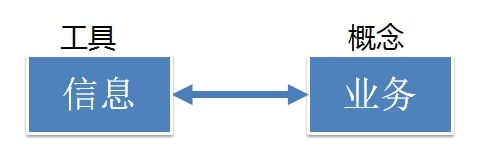
\includegraphics[width=10cm]{Drucker_4tu1_1.jpg}

新的工具逼我们重新思考业务里工作应该怎么做。例如制造业以前都是用传统会计算法,只计算工作的相关成本,比如用机器打磨一个螺丝钉,传统按使用机器工时算成本。但八十年代有ABC
(Activity Based Costing)
作业成本法。就不用传统的视角,它会首先问企业需要做这工作吗?如果需要,好在哪里?然后作业成本法把相关的几个活动,如:价值分析、流程分析、质量管理、成本计算等一起分析,然后有哪些成本的关键要素,再依据实际生产数据,计算合理成本。用了这个新的方式,很多制造业能更合理地做成本分摊,产品定价更合理。但如果制造业公司没有电脑,无法做
ABC,只能用传统的成本会计法。(详见附件)

要利用好新的信息工具来提高管理,不能仅靠IT技术人员领导这场信息革命,还需数据或信息应用管理者合作实现这场革命。

\framebox{%
\begin{minipage}[t]{0.97\columnwidth}\raggedright
\hypertarget{ux5370ux5237ux4fe1ux606fux9769ux547dux7684ux7ecfux9a8cux6559ux8bad}{%
\subsubsection{印刷信息革命的经验教训}\label{ux5370ux5237ux4fe1ux606fux9769ux547dux7684ux7ecfux9a8cux6559ux8bad}}

1500 -
1580年间,懂印刷技术的印刷技术人员非常值钱、成为当时的贵族。但到了1580年左右,他们就变回普通技术人员。\\
现在信息革命也一样:
以前公司里的信息技术人员很昂贵,简称CIO,从以往印刷的历史预测CIO会变成"配角",而不再是``超级明星''。\strut
\end{minipage}}

所以德鲁克先生认为(从管理者的角度)新一轮的信息革命其实还未开始。下面我们看:

\begin{enumerate}
\tightlist
\item
  需要那类信息?
\item
  如何整理信息?
\item
  怎样利用度量计划?
\item
  如何从数据到行动?
\end{enumerate}

\hypertarget{ux7528ux6765ux4e86ux89e3ux4e1aux52a1ux73b0ux72b6ux76844ux7c7bux4fe1ux606f}{%
\subsection{用来了解业务现状的4类信息}\label{ux7528ux6765ux4e86ux89e3ux4e1aux52a1ux73b0ux72b6ux76844ux7c7bux4fe1ux606f}}

企业的主要目的并非控制成本,而是创造价值/财富,所以除了基础信息(
包括如:现金流、项目延误、问题、客户发现缺陷等),要了解现状,还需要对其他3类信息问下面的问题:

\begin{enumerate}
\tightlist
\item
  核心能力 (Competence information)
\item
  生产率 (Productivity)
\item
  资源分配 (Resource allocation information)
\end{enumerate}

\hypertarget{ux6838ux5fc3ux80fdux529b}{%
\subsubsection{核心能力}\label{ux6838ux5fc3ux80fdux529b}}

有什么独特的优秀竞争力?\\
例如,2000年,当谷歌还是起步阶段,
他们就明确定位自己是搜索引擎专家,有别于当时比它庞大的portal公司,如雅虎、AOL。

\hypertarget{ux751fux4ea7ux7387}{%
\subsubsection{生产率}\label{ux751fux4ea7ux7387}}

是否知道自己的生产率。 各不同部门/团队的生产率?与同行业界怎么比?

\framebox{%
\begin{minipage}[t]{0.97\columnwidth}\raggedright
\textbf{标杆}(benchmark)是获取生产率信息的最新工具。这种方法将企业自己的绩效与业内最佳的或世界上最佳的绩效放在一起进行比较。标杆假设一个组织能做的事情,任何其他组织都应做到。它认为任何企业都需要具有全球竞争力,前提条件是至少与领先者做得一样好。
\strut
\end{minipage}}

\hypertarget{ux8d44ux6e90ux5206ux914d}{%
\subsubsection{资源分配}\label{ux8d44ux6e90ux5206ux914d}}

是否适当地投放宝贵资源(如,技术骨干)?\\
内部项目如何立项?\\

\framebox{%
\begin{minipage}[t]{0.97\columnwidth}\raggedright
\vtop{\hbox{\strut \textbf{不良例子}:什么项目都接,只要不亏钱就可以,但未考虑这些项目是否会占用了宝贵资源、会影响到机会成本,长远来看其实对公司不利。}\hbox{\strut \textbf{优良例子}:立项时就考虑是否跟公司的竞争力方向配合。例如一些政府部门及工程的项目对我们核心产品发展没有帮助,我们宁愿不接。谷歌在成立后都有个规定,让每个工程师利用自己20\%的时间选一些他们觉得有前途、对的公司有帮助的项目来做。把公司20\%的资源投入到创新。}}
\strut
\end{minipage}}

\hypertarget{ux5982ux4f55ux6574ux7406ux516cux53f8ux4fe1ux606fux5982ux5ea6ux91cfux6570ux636eux7ecfux9a8cux6559ux8bad-ux77e5ux8bc6ux5206ux4eab}{%
\subsection{如何整理公司信息------如度量数据、经验教训 、
知识分享}\label{ux5982ux4f55ux6574ux7406ux516cux53f8ux4fe1ux606fux5982ux5ea6ux91cfux6570ux636eux7ecfux9a8cux6559ux8bad-ux77e5ux8bc6ux5206ux4eab}}

\hypertarget{ux5ea6ux91cfux8ba1ux5212}{%
\subsection{度量计划}\label{ux5ea6ux91cfux8ba1ux5212}}

要提供工作所需的信息,管理人员首先需要问自己以下两个问题:\\
``我应该向与我共事的人和我信赖的人提供什么样的信息?以什么形式?在多长期限内?''\\
``我自己需要什么样的信息?由谁提供这些信息?以什么形式?在多长的期限内?''\\
最终数据是用来沟通 - 所以团队要问自己需要提供什么数据信息给上级。
例如,生产率质量等。 上层也同样要明确自己需要收集什么数据帮助管理。\\

\hypertarget{ux4eceux6570ux636eux5230ux884cux52a8}{%
\subsection{从数据到行动}\label{ux4eceux6570ux636eux5230ux884cux52a8}}

要解答以上问题,管理者首先要弄清楚度量的目的。

\framebox{%
\begin{minipage}[t]{0.97\columnwidth}\raggedright
如果你没有具体目的地,地图帮不了你。\strut
\end{minipage}}

人们常常认为大量的数据就等同于信息,好像有了厚厚的城市电话簿,我们可能想要的不是电话簿,而是要知道谁想找谁、他的姓名或职业是什么以及他们为什么要通话。

管理者需要了解两件事:剔除与所需的信息无关的数据;整理、分析和解释数据,然后根据获得的信息采取行动。信息的目的不是掌握信息,而是能够采取改进行动。\\
收集数据的目的是让我们可以利用数据做分析,找出根本原因,做改进,不仅仅为了监控。\\

\framebox{%
\begin{minipage}[t]{0.97\columnwidth}\raggedright
例如开发部的目标是降低系统测试缺陷率,可利用
GQM(goal-question-metric)来找出一些会影响结果的度量来帮我们更好控制结果:

G 目标: 降低系统测试缺陷率,减少返工,提高效率。

Q 问题:
有哪些影响因素?是否跟项目类型相关?代码静态检测缺陷率相关?受需求变化频率影响?

针对这些可能因素,收集相关数据来分析:

M 度量: 项目种类、静态检测缺陷率、需求变化频率等\strut
\end{minipage}}

GQM
可以帮我们选择收集哪些数据,收集了足够历史数据后,便可以分析,判断哪些是影响因素。\\

\hypertarget{ux5173ux952eux4e8bux4ef6}{%
\subsubsection{关键事件}\label{ux5173ux952eux4e8bux4ef6}}

如果希望整个企业从上到下实现数字化管理,
便要考虑层次之间的关系,从整个企业的业务目标出发,分解到事业部,最终到团队目标。

每一个层次,关心的形式不一样,如金字塔一样,高层最关心不可能是某个项目的进展,而是整个公司,尤其是对外的那些信息;但中下层或者团队关心的就是项目本身的一些信息。每个层次之间需要充分沟通,所以这些信息之间必须关联起来,高层才可以获得他们要的信息,底层也可以从这个关系知道高层的方向与要求,但这种上下信息的互通很依赖系统支持。\\
如果下面的团队不理解高层的目标,团队各有自己的方向,肯定不会有效果。
反之,上层制定长远战略目标时,如果没考虑下面团队现状,也没有监控下面的进展,这些目标也只是梦想,无法实现。


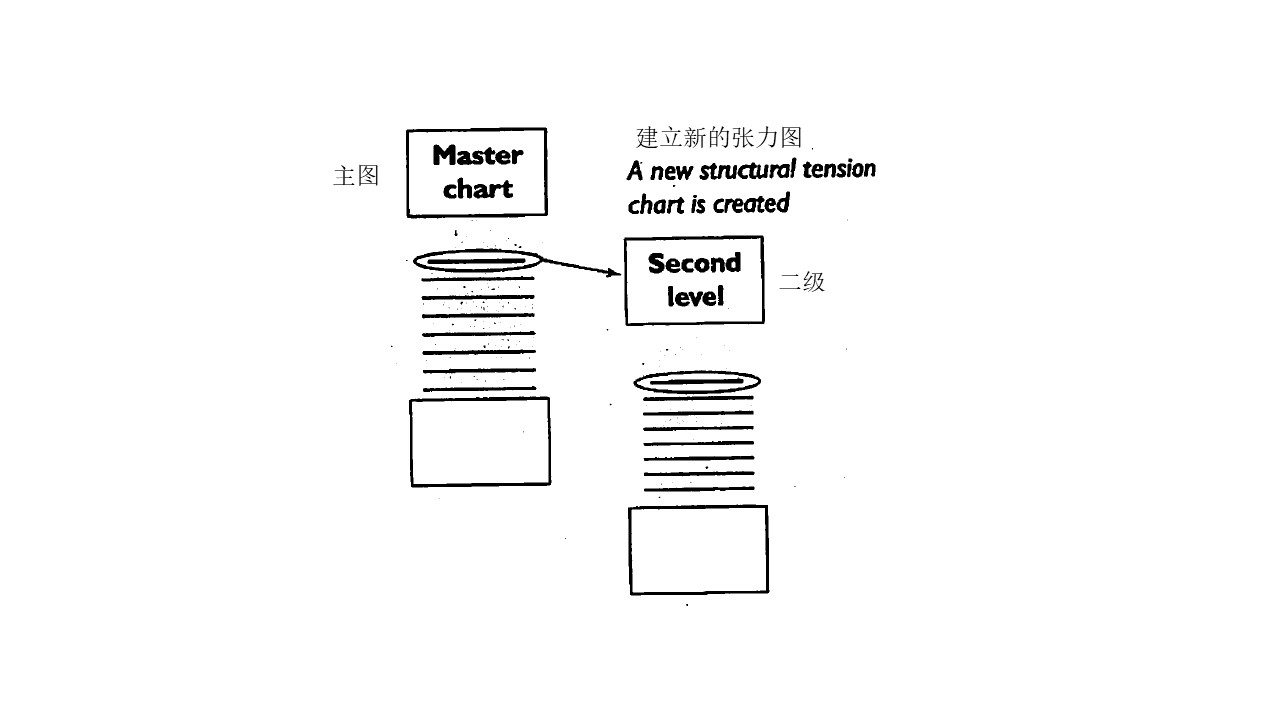
\includegraphics[width=10cm]{Fritz_diagrams_4.jpg}


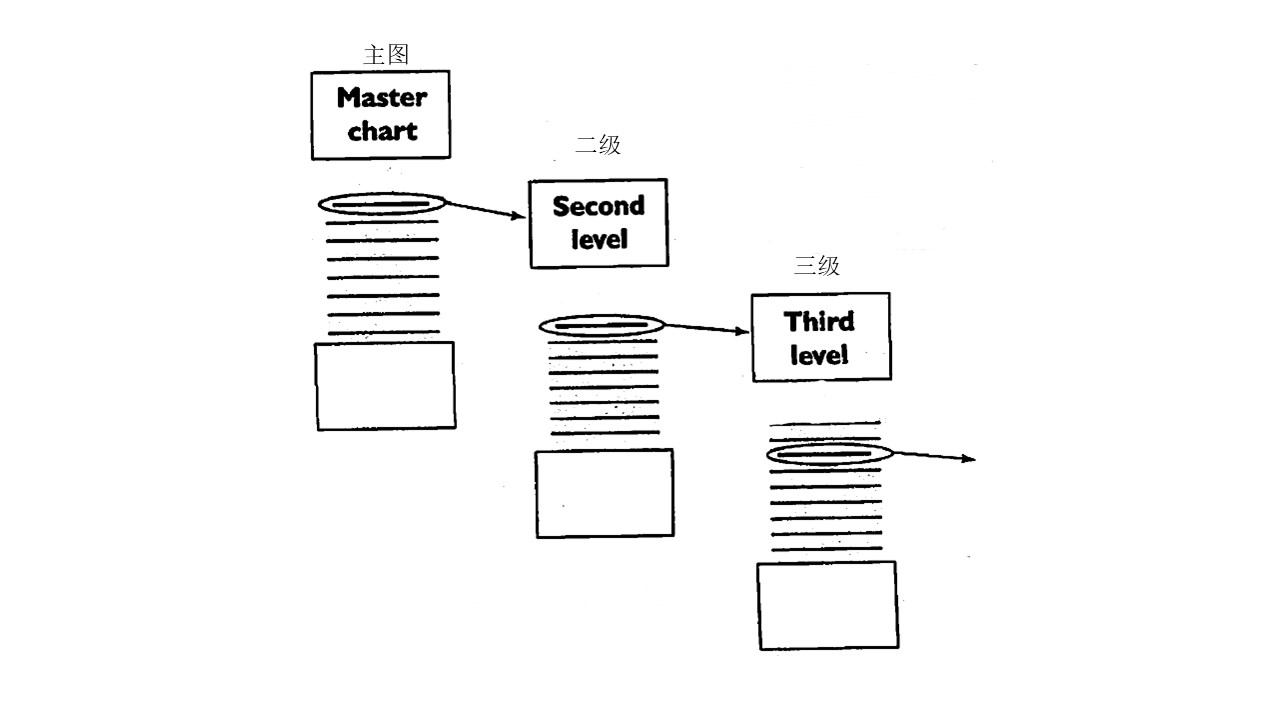
\includegraphics[width=10cm]{Fritz_diag5.jpg}


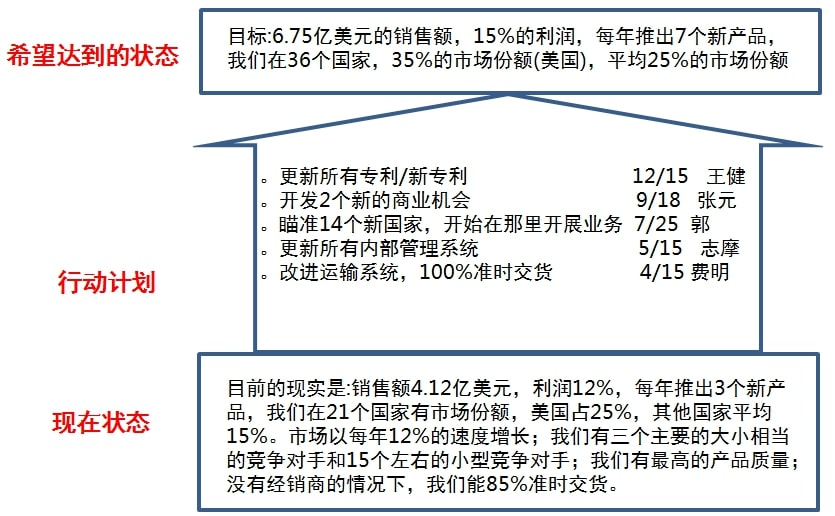
\includegraphics[width=10cm]{Drucker_4_tu3.jpg}

例如上图,高层希望提升销售额、利润,增加新产品等战略目标,必须要有开发团队的支持,如:控制交付后软件产品的质量,软件开发的生产率-每季度可以开发出多少新产品等,目标配合。

\hypertarget{ux5bf9ux8f6fux4ef6ux5f00ux53d1ux7684ux542fux53d1}{%
\subsection{对软件开发的启发}\label{ux5bf9ux8f6fux4ef6ux5f00ux53d1ux7684ux542fux53d1}}

可以用成熟度逐步完善,从基本(1)到可预测(3),让软件开发企业按部就班改善信息化管理:

\begin{enumerate}
\tightlist
\item
  基本项目管理
\item
  项目规模估算
\item
  分析项目历史数据建立基线(标杆)和预测模型
\end{enumerate}

\hypertarget{ux57faux672cux9879ux76eeux7ba1ux7406}{%
\subsubsection{1.基本项目管理}\label{ux57faux672cux9879ux76eeux7ba1ux7406}}

很多软件开发公司,缺乏基本项目管理系统 -\/-
包括项目工作任务分解,管理活动之间的依赖关系,记录在系统中,监控:实际与计划对比,是否延误或者工作量超支。

如果有这些信息,管理者便不用等到项目结束才知道项目是否有问题。

有开发经验的管理者会认为:``我每天都会跟开发团队接触,很清楚每个项目的进展与风险。不需要额外的信息系统帮我管理项目。''

也正是这个心态,妨碍了公司的健康发展,用刚才那个亲力亲为的管理模式,管理者管一百、两百开发人员勉强可以,但可以扩到五百六百已经很难。一千以上规模更不用想。但是反过来看,如果没有合理的信息系统,管理者凭什么去知道项目的风险,哪里会有重大问题?哪些项目质量不好?很可能等到客户投诉才得知。

\hypertarget{ux4eceux4f30ux7b97ux5f00ux59cb}{%
\subsubsection{2.从估算开始}\label{ux4eceux4f30ux7b97ux5f00ux59cb}}

估算缺乏依据,例如:很多项目经理只依赖个人经验估算项目工作量,以为项目的人天数就等同项目规模大小,不理解估算人天数时,已经假定了团队的生产率,所以应先估算项目规模,然后再依据团队生产率估算工作量。

如果要比较不同项目,必须依赖项目规模大小做归一
(Normalize),例如:我们不能用项目缺陷数来比较质量,必须用缺陷率(缺陷数/项目规模)。

在软件开发,如何估算项目规模一直是个挑战,大部分项目开始时无法知道详细需求,便很难用传统功能点分析来估算规模。
迭代项目可以在每个迭代采用简化功能点估算没迭代的规模,后面当需求更清晰时再更新总体功能点估算。(因大部分软件开发项目都采用敏捷迭代方式,不是传统瀑布式,大部分软件开发团队都可以用)

\framebox{%
\begin{minipage}[t]{0.97\columnwidth}\raggedright
功能点估算主要适合用于数据库、交易类软件开发项目,所以大部分软件开发项目都适用,也可参考行业数据基线作参考。

功能点数是一种估算项目大小的指标
(proxy),帮助我们估算项目的工作量进度、缺陷数等。

所以我们收集到项目数据后,需要分析这些项目参数是否与功能点数成线性关系,判断proxy是否确实能准确估算。\strut
\end{minipage}}

对于那些不可以用功能点的项目应如何估算?可以选择其他指标
(proxy),但也需要用项目数据验证。

\framebox{%
\begin{minipage}[t]{0.97\columnwidth}\raggedright
如果做一个全新项目,没有任何历史经验,第一两个迭代,只能依赖专家估算每一迭代的生产率与缺陷率。

但后面迭代的工作量与工期可利用前面迭代的实际数据来估算。

实例:\\
一个大客户希望在5个月内,对总共超过200个各类应用软件做``容器化''自动发布。
项目的总预算和工期已经固定。 乙方项目团队超过20人。
项目经理先与客户协商挑选一些''安全''的应用软件放在第二轮迭代先尝试。
(第一轮迭代,先做基础平台建设准备。)
这项目后面迭代(从第三轮开始到最后第六轮)的估算都会依据第二轮的生产率数据。
也从第二轮迭代经验,优化流程, 调高后面迭代的生产率系数。

虽然前面的迭代有超时, 项目最终还能按时完成。

这是偏实施的软件开发项目,传统功能点分析不适用,项目组采用传统代码行数为规模指标,从6轮的数据后,也验证代码行数确实可作为
proxy。\strut
\end{minipage}}

\hypertarget{ux57faux7ebfux6807ux6746ux548cux9884ux6d4bux6a21ux578b}{%
\subsubsection{3.基线(标杆)和预测模型}\label{ux57faux7ebfux6807ux6746ux548cux9884ux6d4bux6a21ux578b}}

\hypertarget{ux5229ux7528ux4fe1ux606fux5e2eux52a9ux51b3ux7b56}{%
\subsubsection{利用信息帮助决策}\label{ux5229ux7528ux4fe1ux606fux5e2eux52a9ux51b3ux7b56}}

没有数据就无法比较。

\framebox{%
\begin{minipage}[t]{0.97\columnwidth}\raggedright
有一次问一位下面有5位开发人员的开发组长,问他如何判断开发人员的学习进展,能力是否有提升?

他说:``我们每月都会有考核,多项打分(1-10分),我会每人在这期间是否完成下发给他的任务是否按时完成等打分。''

但他做判断时能否客观?比如下面小李开始时某方面表现较出众,很可能他其他项都普遍高分;反过来小王可能沟通表达能力较弱,会影响其他项打分不高,这是靠人主观判断的常见的误区。但如企业有收集每个开发人员的每周有效代码数、功能点数
(生产率)和一次性通过率(质量)等客观指标,考核便能比较客观,也能让个人和团队实时知道是否有改进。\strut
\end{minipage}}

好比锻炼跑步,目标想跑马拉松。
如果一直都没有收集跑步的数据,肯定很难有任何提升。
软件开发也一样,第一个挑战是如何让个人与团队开始有定期一两周收集数据的习惯。
开发工程师都是公司核心骨干,很有自己的想法。
必须让他们觉得数据有用,才愿意去做。
所以,我们会用一些互动练习,模拟项目组冲刺后做回顾。
让他们感受感受到有数据,并形成柱状图,趋势图等的讨论,比以前但依赖每人发表意见讨论更有效。

这种以数据监控团队效率/服务的管理方式,其实已经一直在很多服务业使用(如呼叫中心,每个团队的头顶都会有数字大屏,实时反映这个团队的平均解决客户问题时间,客户投诉率等。)也正是有了这些客观数据,才能激励团队想尽办法改进团队的成绩,不能比其他团队差。

信息只是一个工具,更关键的是背后的概念和业务本身,如果有了这些新的数据信息,是否可以帮我们更好做业务才是最关键。

软件开发的度量不仅仅能帮助团队和个人持续改进,也能帮管理者做决策。

例如软件项目报价。有一家公司各省的都有分公司,分公司主要谈业务接单,总部做开发。为了抢单,业务员都会尽量把压低软件价格,导致还未开工,项目经理就已经知道无法在预算内完成。

如果有收集以往同类项目历史数据,项目经理就可以估算项目工作量。请注意,我们没有说项目的报价,就是完全按照系统历史数据估算,业务变化万千,可能是战略需要,亏本也要接这个单,因为他可能会开拓后面附加业务。但有了这个历史数据的项目估算信息,管理者便可估计项目会亏多少,不会等到接单后才知道。

如果企业有不断收集项目数据,形成标杆,不断更新基线,企业便可以利用基线或者标杆去帮助知识工作者持续改进。

项目信息不仅仅是把项目管理从六十分提高到八十分,而是企业的最基本竞争力。刚才这个例子也可以扩大,不仅仅是用于一些投标客户定制化开发项目。如果公司是做软件产品也一样:
如何定产品的卖价,以前都是一门``艺术'',只有CEO或业务经理才知道,他也说不出来按怎么去定价,反正公司就活下来。但是如果我们有了那些项目的信息知道我们平均开发一个新的功能点要多少开发成本,对产品经理是很重要的信息,如何定软件产品的卖价的考虑因素。

正如德鲁克先生在九十年代的观点,就算你是一个传统的经理人,生意人主要是关注买卖,低价买入,高价卖出,要盈利。你可以想象量化管理如果做好,也可以帮到你。更深入去想,这个内部管理的信息化是一个很重要的企业竞争力。只是现在你的同行大部分都在睡梦中没有醒过来,当你发现他们醒过来才反应的时候,可能已经为时而晚了。

你可能会说:``你说这些都正确,但是我们还没到这个地步,暂时不需要像你说的那种推行量化管理。''\\
软件开发人员常会有一个误解:``我们跟那些大企业不一样。我们是无法像这种用数据做估算和计划,因软件开发变数太多。''\\

\hypertarget{ux5e94ux5982ux4f55ux5f00ux59cb}{%
\subsubsection{应如何开始}\label{ux5e94ux5982ux4f55ux5f00ux59cb}}

了解为何要度量? 改进目标?
为了让团队认同度量的重要性,我们会先把企业所有干系人聚在一起,开2天半的工作坊,辅导他们讨论公司战略目标,有哪些改进方向?如何利用数据做回顾,根因分析,让每个团队一起定度量计划,为了满足公司的发展需要,如何收集哪些数据,哪些因素会影响团队的质量与生产率?例如,如觉得代码质量可能是主因,要收集哪些指标来衡量代码质量?经过工作坊过后,我们会按生产率与质量两目标,做2天针对性地培训,教他们如何从需求可以估算功能点数、工作量,辅导他们利用数据模板,开始每2周收集项目信息。

我们4年前开始辅导团队如何使用简化功能点方式估算迭代的规模。我们的客户都能经过两天培训后便开始使用这方法开始收集项目迭代生产率数据。

建立基线\\
当企业团队、软件开发团队一直有收集以上的基本数据,我们就发现它们之间都有一个相对稳定的比例。有些可能会跟不同的客户方的业务有差异,例如你做一个高端的银行系统,可能跟一个普通的网购项目有差异,但是我会依据这些基本的差异把基线细分。我们就可以知道你是这类项目,从历史数据按现在需求估出来的项目规模,刚才说的成本进度、代码行数大概多少?我们没有说他非常精确,但起码它会比你单靠个人经验,拍脑袋估算更有参考价值。

\framebox{%
\begin{minipage}[t]{0.97\columnwidth}\raggedright
问:
增加了这么多数据度量和文档准备是否会增加额外的工作导致整体效率降低?
答:所以我们只收集关心的和用来分析的数据;例如我们一个迭代收集的数据都不超过15个,都是最基本的。如企业觉得不够,才增加。\strut
\end{minipage}}

``你是否要很高深的统计学概率等基本知识才做得到?''

管理者/项目经理,其实只需要懂得如何利用这些统计分析的结果,改善项目管理,不需要量化统计学专家。现在科技发达,有很多现成的分析工具,如果企业能累积到充分和准确数据,分析不困难。

最困难是如何让知识工作者有动力/有兴趣收集数据。
与制造业不一样,数据必须要由知识工作者提供。
如果他们不觉得提供这些数据对工作有帮助, 他们肯定不愿意。

就算公司规定,
如果他们不相信度量这些有用,他们很可能随便填报,公司也没办法。
所以数据是否被使用帮助团队做改进非常重要。

如果没有数据,冲刺后的团队回顾,大家都利用分析本冲刺的数据,如缺陷数分布,源于以往历史数据比较。
一起讨论找出根本原因在上一个从此采取改进行动,每个团队成员很自然会积极提供数据。

反之,冲刺大会没有任何项目数据,只是大家坐在一起讨论头脑风暴。
冲刺回顾会逐渐会变成内部``批判会''失去动力参加回顾。

公司积累了一定数量的数据后,比如\textasciitilde{} 70 - 100 组数据。
便可以做统计分析,并建立公司基线 和 预测模型。
如果公司有做数据,挖掘,大数据等服务,其实数据分析的方式类似。
经理,过程改进组长和项目经理不须熟悉统计分析,但他需要知道如何利用这些数据分析结果,帮他们做好量化项目管理与根本原因分析。

度量计划很关键,因信息化管理必须收集合适的数据。例如,有些管理层只关注项目进度是否延期,但不监控项目的质量(各类缺陷密度)。只关注结果,不关注过程。如果开发的质量不理想,大量缺陷导致很多返工,项目的结果(进度偏差)肯定不会好到哪里?

企业要信息化管理,不是简单一两个月便能完成。
所以必须有一个项目计划,有里程碑才会有效果。
但每个项目组都特别忙,没时间,怎么办?
参加CMMI高成熟度评估,可以使企业有动力订立一个9到12月的改进计划,按部就班地推量化管理。

\hypertarget{ux603bux7ed3}{%
\section{总结}\label{ux603bux7ed3}}

21世纪整体的环境变化比上一个世纪更快速,企业为了不被最终淘汰,首先必须从信息管理入手,不能再依赖以往经验做决策和管理。\\
你对以上的问题都心里有数吗?如果不是,便应想想如何赶上。\\
软件开发企业的管理改革,与我们辅导开发团队做量化管理如出一辙,都必须基于数据。管理层除了要关注内部团队的效率与质量外,更要重视上面提到的信息。\\
推行企业的变革肯定有难度。首先管理者要不满意现在的度量与分析,才会有动力下定决心去改。因为要成功,肯定不会一步到位,必须经过很多轮的试点,然后调整,才最后有效果。所以高层的决心与支持是成功的必需条件。

下一篇
会从他的2002 文章``他们是人,非雇员They're Not Employees, they're
People`` 谈起,以TQM 系统总结。



\hypertarget{ux9644ux4ef6}{%
\section{附件}\label{ux9644ux4ef6}}

\hypertarget{ux4f5cux4e1aux6210ux672cux6cd5-activity-based-costing-abc}{%
\subsubsection{作业成本法 (Activity Based Costing
ABC)}\label{ux4f5cux4e1aux6210ux672cux6cd5-activity-based-costing-abc}}

生产业越来越多用新科技降低成本,如果还是传统的按使用了多少人时,或用了机器多少时间来计算和分配成本已不能反映真正成本。
如没有一个完善的成本会计方式,管理层是难以知道内部的真正成本,也很难去定产品的合适价位。\\
例如,产品1234,生产量不多。 占用生产机器的时间也短。
但因不能占用生产设备的所有时间。
每次生产都要花精力去准备,完成后也需要再调整,把设备恢复到生产其他产品配置。
另外产品5678,大量生产,占用生产设备的所有时间,所以不需要花精力去准备。
如果按传统会计按占用机器投产工时分摊,大部分的成本都会分到5678产品。
分配到1234产品的成本却很低,并不能反映真正的成本。

针对传统会计不能 合理分摊成本,生产业开始使用ABC:

首先要把识别每一种关键成本因素。
例如,准备生产设备;编写管理生产设备的软件程序;设备占用的地方面积:设备检查次数等。
然后收集实际数据。 花6到12个月时间做ABC对企业的价值包括:

\begin{itemize}
\tightlist
\item
  管理者更了解每个产品的实际成本,定项目产品价
\item
  了解哪些成本效益不高,要针对性完善
\end{itemize}

软件开发虽然没有产品生产这么复杂,但仍要合理分摊复用模块成本。
例如,越来越多公司,使用标准产品和复用模块来增高项目的生产率。
但应如何把复用产品的开发成本分摊到项目中?
例如,如果是按产品开发组的实际工作量计算成本,
销售会说"为什么你的成本这么高,是否你的开发效率低
为什么要我这个项目为你买单?"
所以不能单看工作量,要能真正反映的参数(例如,软件功能点数),
也需要有信息化系统,计算项目实际成本,管理层才可以看得出哪些部分效率低需要完善。

%\begin{description}
%\item[]
%\begin{description}
%\tightlist
%\item[]
%-\/-\/-===\textless{}\textless{}\textless{} END
%\textgreater{}\textgreater{}\textgreater{}===-\/-\/-
%\end{description}
%\end{description}

\cite{drucker1References1}
\cite{drucker1References2}
\cite{drucker1References3}


